\chapter{Technologische Konzeption ( 5\% )}


Im vorhergehenden Kapitel wurde das grundlegende System konzipiert.
Fortsetzend daran sollen nun geeignete Technologien und Werkzeuge gefunden werden,
um einen Prototyp umzusetzen.
Außerdem werden notwendige Anpassungen der Konzepte an technische Gegebenheiten vorgenommen werden,
um die fortf\"uhrende Implementation zu unterst\"utzen.


% begruendet technologie, ist trasnformation notwendig

% evtl kap 7 referenzieren


\section{Datenbank}

Die Auswahl der Datenbanktechnologie und eines darauf basierenden Datenbankproduktes sind die wichtigsten technologischen Entscheidungen dieser Arbeit.
Die im \Cref{chap:design} vorgestellten Lösungen sollen als prototypisches System umgesetzt werden.
Die Datenbank stellt die Basis dieses Systems und ihre Eigenschaften werden die Implementation maßgeblich beeinflussen.


\subsection{Technologische Betrachtung}

%XXX: Bild overview verweisen
In einer initialen Sondierung zeigte sich,
dass 3 Klassen an Datenbanken die grundlegenden Anforderungen an die Modellierung des Denkschemata erfüllen.
Dies sind die Dokument-orientierten Datenbanken, die Graphendatenbanken und moderne relationale Datenbanken. 

\Cref{fig:classen-datenbanken}

\begin{figure}
    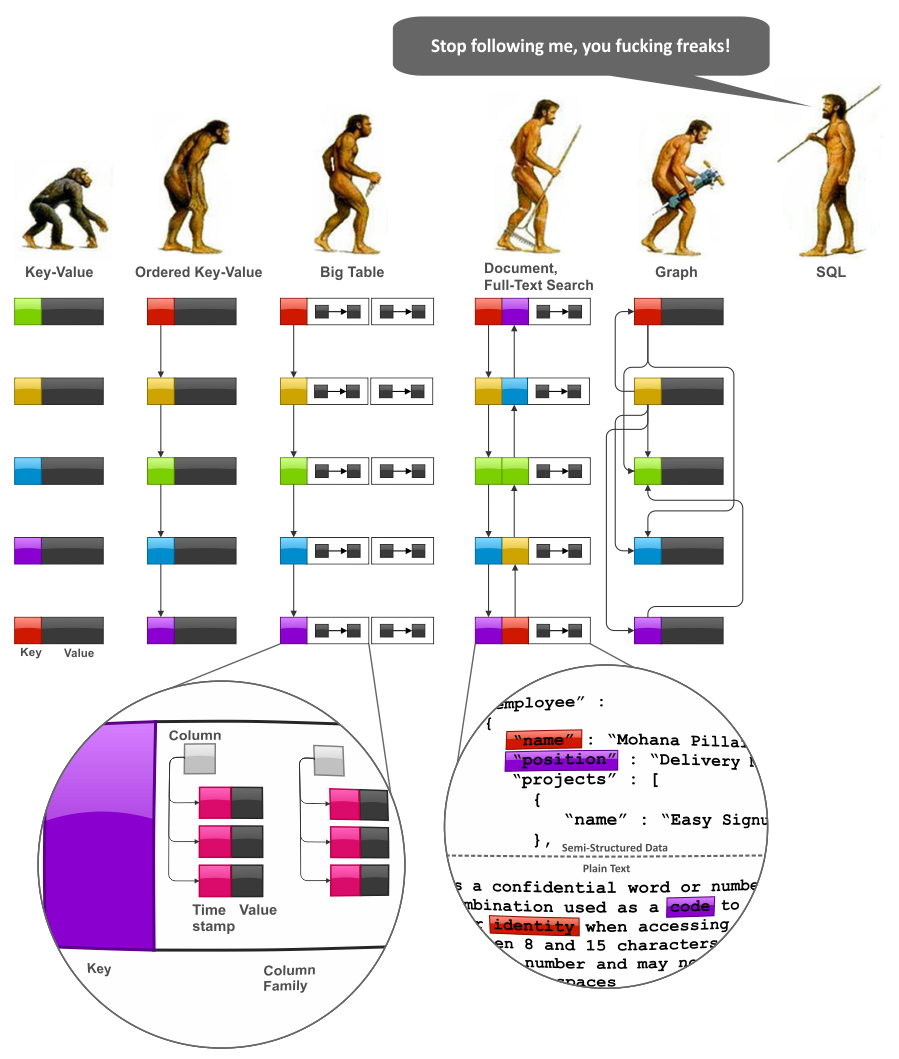
\includegraphics[width=\textwidth]{images/databases-overview.png}
    \caption{Übersicht Klassen an Datenbanken}
    \label{fig:klassen-datenbanken}
\end{figure}

\subsection{Produktanforderungen}

Wie die technologische Betrachtung zeigte,
sind mehrere Arten von Datenbank für die Modellierung geeignet.

Um ein geeignetes Produkt zu bestimmen,
m\"ussen Anforderungen herausgearbeitet werden,
welche sp\"ater bei der Implementation hilfreich sein k\"onnten.

Wichtigstes Kriterium ist dabei, dass die Datenbank tats\"achlich \textbf{verteilt} ist.
Um sicherzustellen, das alle Systemanforderungen erf\"ullt werden k\"onnen,
muss die Datenbank zus\"atzlich \textbf{Master-Master Replikation} beherrschen.
Selbstverst\"andlich muss die Replikation mit einer \textbf{Partitionierung} des Netzwerkes zurechtkommen.

Ein weiteres wichtiges Werkzeug, welches die Datenbank mitbringen sollte, sind \textbf{Mitteilungen über Änderungen}.
Unterschiedliche Komponenten des Systems beginnen mit ihren Aufgaben,
wenn Änderungen an der Datenbank stattfinden.
Daher sind detaillierte Echtzeit-Informationen über Änderungen der Datenbank eine entscheidende Komponente,
deren Einfluss auf Latenzen und Antwortzeiten der Komponenten nicht zu unterschätzen ist.


\begin{verbatim}

- selektive/gefilterte replikation wuenschenswert
- local atomic <> mvcc ?

-> modellierung referenierung
% schemata
% mapping auf datenbank aenderungen

-> couchdb ausarbeiten

\end{verbatim}


\section{Programmiersprachen}

Die Programmiersprachen stellen die Basis f\"ur produktives Entwicken,
sie erm\"oglichen erst die Umsetzung eines Projektes.

\subsection{Technologische Betrachtung}

Da ein Prototyp geschaffen werden soll,
ist eine Programmiersprache mit hoher Produktivit\"at gefragt,
selbst wenn dies auf Kosten von Performance geschieht.

Daher bietet sich die Klasse der Skriptsprachen an,
ihre dynamische Natur ermöglicht es,
in kleineren Projekten schnell zum Ziel zu kommen.
%XXX cite?
Weiterhin muss eventuell die Datenbank-interne Sprache beachtet werden.

% klassen/moduldiagramme aus kap 5 referenzieren

\subsection{Produktanforderungen}

Im Detail sind nur einige wenige Punkte zu beachten.
Die Wahl der Sprache an sich steht frei,
solange bestimmte Bibliotheken verf\"ugbar sind.

Wichtig sind dabei vor allem folgende Punkte.
\begin{itemize}
    \item Datenbankzugriff 
    \item Prozesskontrolle f. Prozess basierte Arbeitsschritte
    \item Zugriff SCM
    \item Automatisches Testen
\end{itemize}

Außerdem sollten der Entwickler bereits mit der Sprache vertraut sein.
Für die Datenbank-interne Sprache muss sich nach der Datenbank gerichtet werden.


\section{Weitere Werkzeuge}

Hier werden weitere Werkzeug-arten und Technologien vorgestellt,
welche die Implementation unterstützen werden.

\subsection{Testwerkzeuge}

Um die noch zu entwickelnden UnitTests,
sowie die bereits in \cref{chap:target} spezifizierten Tests umzusetzen,
is es notwendig Tests zu schreiben. Um diese Aufgabe zu erleichtern
und gleichzeitig 

\subsection{Datenbank Management}

Zur Verwaltung der Datenbank, sowie Datenbank-intene Programmteile,
werden Werkzeuge zum analysieren und verwalten benötigt.


\section{Konzeptuelle Abbildungen}

Diese Sektion behandelt Konzeptuelle Abbildungen der Ideen aus dem Grobkonzept.
Sie sollen den verwendeten Technologien Angepasst werden

\subsection{Ausschreibungsverfahren für die Auftragserteilung}
\label{sec:verfahren:erteilung}
Für die Umsetzung des Ausschreibungsverfahren der Auftragserteilung gibt es
mehrere Möglichkeiten, die Inanspruchnahme eines Auftrages in
der Datenbank umzusetzen. Je nach Fähigkeiten der Datenbank kann man 
alternative Versionen des selben Datenobjekt nutzen,
oder auf separate Datenobjekte, welche die Inanspruchnahme ausdrücken setzen.

\subsubsection{Alternative Versionen}

Bei der Umsetzung mit alternativen Versionen, wird die Technik \textbf{MVCC} (Multiversion Concurrency Control) eingesetzt.
Sinnhaft Übersetzt bedeutet das Kontrolle der Nebenläufigkeit durch multiple Versionen.

Im Prozess der Zuteilung sind dabei mehrere Versionen eines Arbeitspaket Objektes vorhanden und jede Version bringt eine andere Inanspruchnahme zum Ausdruck.

Die eigentliche Zuteilung wird Anschließend diesen Konflikt wieder bereinigen.
Dabei wird eine neue Version des Arbeitspaketes erstellt, welche den Gewinner festlegt und alle anderen ersetzt.
% More?

\subsubsection{Separate Datenobjekte}

Bei der Abbildung als separate Objekte in der Datenbank,
wird für jeden Arbeiter, der ein Arbeitspaket ausführen will, ein $Claim(Packet, Arbeiter)$ erzeugt. Diese bringen Inanspruchnahme zum Ausdruck.
Der Manager kann dann eines dieser Claim Objekte auswählen und dem Arbeitspaket einen Arbeiter zuteilen.
%MORE!

\subsection{Alternativen zu Fabriken in Skript-sprachen}

Das Fabrik-Muster kommt vorwiegend in statisch typisierten Objektorientierten Sprachen zum Einsatz. In dynamisch typisierten Sprachen gibt es jedoch eine weitere Methode, das Dynamische Instantiieren von Abgeleiteten Klassen zu behandeln.

Anstelle einer Fabrik-klasse, die Konfiguriert wird,
kann eine einfache Zuordnung an Konstruktoren anlegt werden.

Dies trifft besonders auf die ``Proc'' Klassen (Siehe \Cref{fig:klassen-arten-arbeitsschritt}) zu.
Ihre Zuordnung zu Arbeitsschritten findet über den Wert eines Attributes statt
daher ist eine eindeutige Zuordnung über ein Mapping ausreichend.

\begin{figure}
\begin{minted}{python}
#pseudocode
class Proc(object):
    def __init__(self, lookup):
        ...
        self.lookup = lookup or default_lookup()

    def run(self, step):
        proc = self.lookup[step.stepper](self, step)
        proc.run()
\end{minted}
\caption{Beispiel Zuordnung statt Fabrik}
\end{figure}